\documentclass[10pt,letterpaper]{article}
 \usepackage[utf8]{inputenc}
 \usepackage[spanish]{babel}
 \usepackage{amsmath}
 \usepackage{amsfonts}
 \usepackage{amssymb}
 \usepackage{graphicx}
 \usepackage[left=2cm,right=2cm,top=2cm,bottom=2cm]{geometry}
 \usepackage{float}
 \author{}
 \setlength{\parindent}{0cm}
 \title{Programación avanzada y métodos numéricos.}
 \date{}
 
 \begin{document}
 \begin{center}
 \LARGE {\textbf{Programación avanzada y métodos numéricos.}}\\
 \end{center}
 \begin{center}
 Claudio Aravena Plaza. 
 \end{center}
 Viernes 13 de julio de 2018. \hfill Profesor: Benjamín Toledo. \\
 Problema 4. \hfill Ayudante: Diego Ibarra. \\
 
 
 
 
 \begin{enumerate}
\item \textbf{Descripción del programa.}\vspace{0.3cm}\\
\small El programa tiene como función realizar una clase de matrices que cuente con las operaciones básicas, ya sea, la suma, resta, multiplicación por izquierda y por derecha, cargadas como operadores además de otras como la función traza. La clase fue traspasada a plantilla, lo que las funciones y los operadores definidos aceptan cualquier tipo de variable. Se sobrecargaron algunos operadores propios de las operaciones descritas anteriormente, además del operador asignación $=$. 

\begin{enumerate}
\item[1.3]\textbf{Definición de la clase}\\
\small La clase de matrices tendrá como variable privada un vector objeto importado desde STL, y tres número enteros que representaran el número de fila(f), número de columnas(c) y el producto de ambos denotado como ``dim''. En la figura 1 se puede observar el código que representa esto.

\begin{figure}[H]
\begin{center}
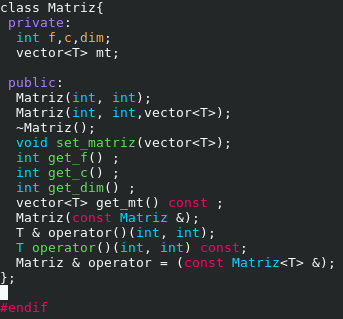
\includegraphics[scale=0.4]{definicion_clase}\\
\textbf{Figura 1.} Extracto de código de definición de la clase. 
\end{center}
\end{figure}
Además el contructor tiene la siguiente estrucutura 

\begin{figure}[H]
\begin{center}
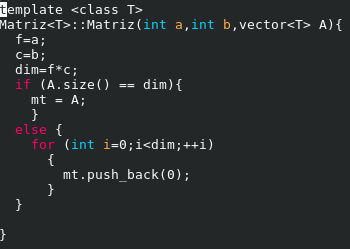
\includegraphics[scale=0.4]{contructor}\\
\textbf{Figura 2.} Extracto de código del contructor de copia. 
\end{center}
\end{figure}



\item[1.2] \textbf{\small ¿Cómo transformar la información de un vector en un arreglo?}\\
  \small La pregunta es como se puede representar la información contenida en el vector, como una matriz con filas y columnas. Para ejemplificar la forma se considera una Matriz cuadrada de dimensiones $2\times 2$,
  \[A=\left( \begin{array}{ll}
               a_{0.0}& a_{0.1}\\
               a_{1.0}& a_{1.1}\\
             \end{array}\right).\]
         
        \small  La matriz a cada componente le asigna dos valores, el primer subíndice corresponde al número de filas y el segundo al de columnas. Entonces los elementos se guardaran en el vector de la siguiente manera
        \[ v=(a_{0.0},~a_{0.1},~a_{1.0},~a_{1.1}).\]
        El primer problema por resolver es encontrar un algoritmo que muestre algún elemento de la matriz que se le solicite a través de alguna función o algún operador. Como los elementos están ordenados, tienen un par ordenado que los indentifica. Si se pide el elemento $A_{i.j}$ la idea es determinar donde se encuentra dentro del vector. Para este caso la respuesta es simple ya que el elemento $A_{i.j}$ estaría almacenado un número $c$ de posiciones (número de columnas) hacia la derecha de donde está $A_{i-1.j}$. Para el ejemplo esta idea es correcta porque es el elemento $A_{1.0}$ se encuentra en la tercera posición del vector. Para esta función se sobrecargó  el operador ``()''.\vspace{0.2cm}\\
        Ahora ya conociendo como llamar a cada elemento de la matriz desde el vector que la genera, se debe crear un ciclo que recorre los coeficiente en orden para de esa forma representarla. Es decir, se hizo un ciclo for recorriendo números naturales hasta un largo igual al número de fila  y dentro de este, otro que recorre número naturales hasta un largo equivalente al número de columnas. Tal como se observa la figura 3.
        

\begin{figure}[H]
\begin{center}
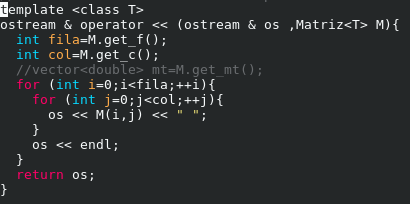
\includegraphics[scale=0.4]{cout}\\
\textbf{Figura 3.} Extracto de código de representación de la matriz. 
\end{center}
\end{figure}


\item[1.3] \textbf{Multiplicación de matrices}\\
  Las operaciones suma, resta, y multiplicación escalar son equivalentes a sumar, restar y multiplicar respectivamente término a término los elementos del vector que contiene los elementos de la matriz. Ahora la multiplicación de dos matrices resulta un problema adicional. Si se toman dos matrices $A$ y $B$, el resultado es

  \[AB=\left( \begin{array}{ll}
               a_{0.0}& a_{0.1}\\
               a_{1.0}& a_{1.1}\
             \end{array}\right)\left( \begin{array}{ll}
               b_{0.0}& b_{0.1}\\
               b_{1.0}& b_{1.1}\\
             \end{array}\right)=\left( \begin{array}{ll}
               a_{0.0}b_{0.0}+a_{0.1}b_{1.0}& a_{0.0}b_{0.1}+a_{0.1}b_{1.1}\\
               a_{1.0}b_{0.0}+a_{1.1}b_{1.0}& a_{1.0}b_{0.1}+a_{1.1}b_{1.1}\\
                                       \end{array}\right)\]

                                   Para poder reproducir esta idea, se pueden hacer ciertas observaciones: Si la matriz $A \in M_{m\times n}$ y la matriz $B \in M_{n\times p}$ entonces el producto puede espresarse $$AB_{ij}=\sum_{k=0}^{n} A_{ik}\cdot B_{kj} .$$ Para realizar esto se deben tomar 3 ciclos for anidados, corriendo los índices de cada elemento. El primero debe se debe terminar cuando existan un número $m$ de elementos. El segundo deberá correr hasta tener un número $p$ de elementos y el tercero hasta tener un número $n$ de elementos.
                                    
\begin{figure}[H]
\begin{center}
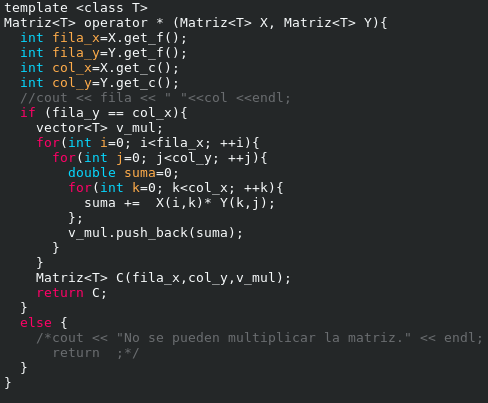
\includegraphics[scale=0.4]{multiplicacion}\\
\textbf{Figura 4.} Extracto del código para el operador multiplicación de matrices. 
\end{center}
\end{figure}
Este algoritmo representado en la figura 4, entrega resultados correctos para todos los casos posibles incluso para cuando se pretende multiplicar tanto por la izquierda como por la derecha.

\end{enumerate}


\item \textbf{Ejemplo}\\
Como ejemplo se realizarán representaciones de dos matrices $M$ y $G$, además se realizaran dos operaciones que agrupan las operaciones elementales, incluso se hace multiplicación por derecha y por izquierda. 

\begin{figure}[H]
\begin{center}
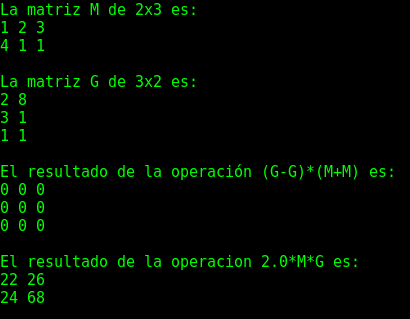
\includegraphics[scale=0.3]{ejemplo}\\
\textbf{Figura 5.} Output de salida desde la terminal de los ejemplos ejecutados.  
\end{center}
\end{figure}
  

\end{enumerate}
 \end{document} 
